\documentclass{book}
\usepackage{booktabs}
\usepackage{geometry}
\usepackage{enumerate}
\usepackage{setspace}
\usepackage{amsthm}
\usepackage{float}
\usepackage{color, soul}
\usepackage{amsmath,amssymb}
\usepackage{amstext}
\usepackage{makecell}
\usepackage{graphicx}
\usepackage{array}
\begin{document}
{\huge 4.1 Projectile motion with air drag}

{\Large 1.}
\vspace{0.01\textheight}
According to Newton's Second Law:

$\begin{cases}
    V_{x_{0}}= & V_{0}cos\alpha \\

    V_{y_{0}}= & V_{0}sin\alpha
  \end{cases}$
\quad $
  \begin{cases}
    a_{x_{i}}= & -\frac{k}{m}v_{x_{i}}   \\

    a_{y_{i}}= & -g-\frac{k}{m}v_{y_{i}}
  \end{cases}
$

\vspace{0.03\textheight}
Using Euler's method:
\vspace{0.01\textheight}

\quad $
  \begin{cases}
    v_{x_{i+1}}= & v_{x_{i}}+a_{x_{i}}\Delta t = v_{x_{i}}(1-\frac{k}{m}\Delta t)           \\

    v_{y_{i+1}}= & v_{y_{i}}+a_{y_{i}}\Delta t = v_{y_{i}}(1-\frac{k}{m}\Delta t)-g\Delta t
  \end{cases}
$

\vspace{0.01\textheight}

\quad $
  \begin{cases}
    x_{i+1}= & x_{i}+v_{x_{i}}\Delta t \\

    y_{i+1}= & y_{i}+v_{y_{i}}\Delta t
  \end{cases}
$

\vspace{0.01\textheight}
{\Large 2.}
The initial conditions are set as: $x_{0}=y_{0}=0, \alpha =\frac{\pi}{6}$.

\quad The numerical result is given as:

\quad $\begin{cases}
    x(t)= & v_{0}cos\alpha \cdot \frac{m}{k}(1-e^{-\frac{k}{m}t})                          \\
    y(t)= & (v_{0}sin\alpha + \frac{mg}{k})\frac{m}{k}(1-e^{-\frac{k}{m}t})-\frac{mg}{k}t)
  \end{cases}$

With the analytical formulas and numerical values, four trajectories are plotted as belows:

\begin{figure}[h]
  \centering
  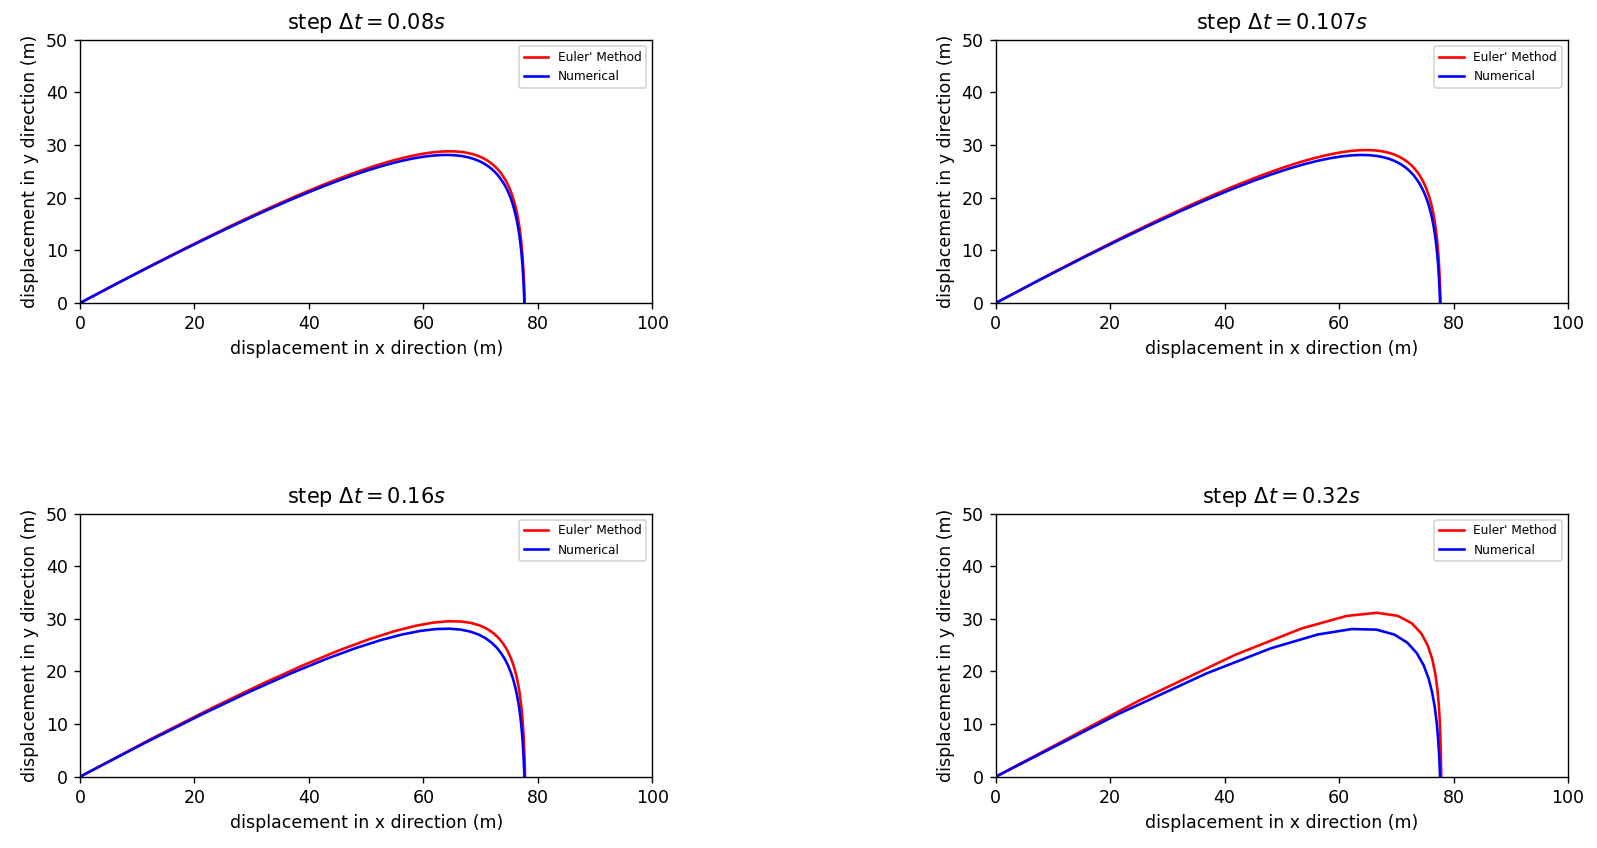
\includegraphics[width=12cm,height=6cm]{project4.1.2.png}
  \caption{4.1.2. Plot the trajectories}
\end{figure}

\newpage
{\Large 3.(a)}
\begin{figure}[H]
  \centering
  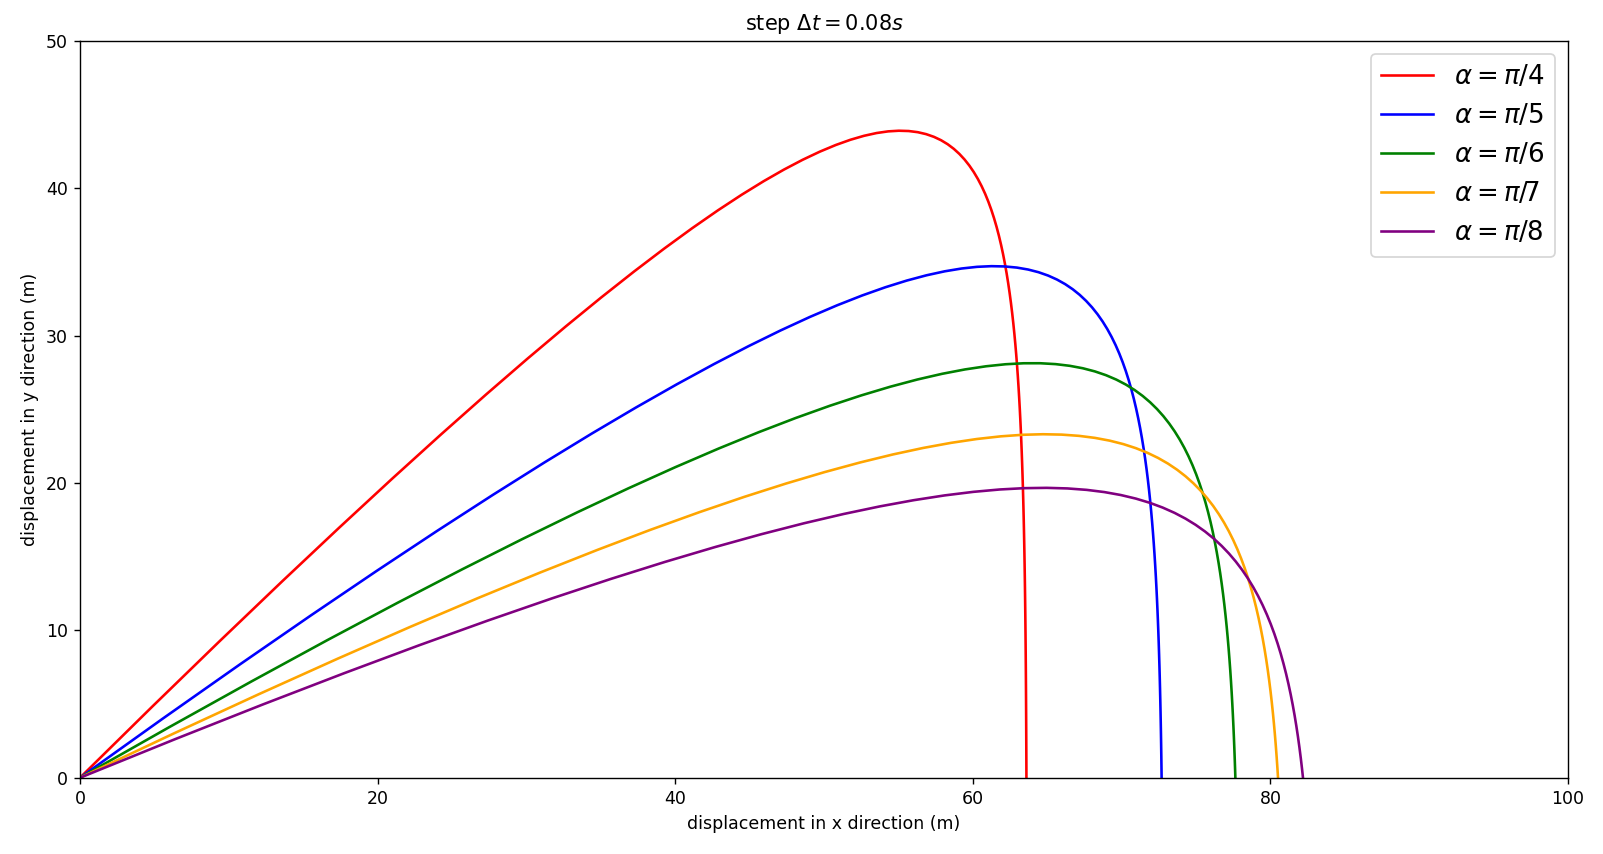
\includegraphics[width=12cm,height=6cm]{project4.1.3(a).png}
  \caption{4.1.3(a). Plot five trajectories for differenct initial angles}
\end{figure}
Choose the step to be 0.08s.
The initial speed of the projectile is fixed to be 90m/s, and the problem is solved numerically for five different values of angles.
  {The five angles are selected to be $\frac{\pi}{4},\frac{\pi}{5},\frac{\pi}{6},\frac{\pi}{7},\frac{\pi}{8}.$}, and the graph is shown in Figure 2.

The shape of the trajectories are quite similar as all of them increasely steadily and then precipitate sharply.
It can be observed the figure that, the larger the initial angle to the horizontal is, the higher the maximum height is, and the shorter the range is.

\vspace{0.004\textheight}
{\Large 3.(b)}
\begin{figure}[H]
  \centering
  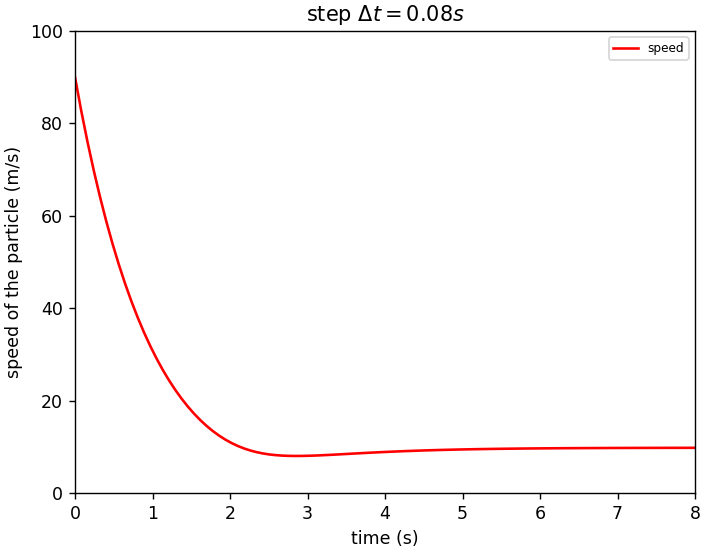
\includegraphics[width=9cm,height=6cm]{project4.1.3(b).png}
  \caption{4.1.3(b). Plot the time dependence of the speed of the particle}
\end{figure}
It can be observed from the graph that, the speed of the particle drops quickly at the first several seconds, and then the speed become stable.
\end{document}